\documentclass[a4paper,openright]{memoir}

\usepackage{prelude/lhs2TeX}

\title{Ghengin: A type-heavy, shader-centric Haskell game engine}
\author{Rodrigo Mesquita}

\begin{document}

\maketitle

\chapter{Ghengin}

\section{Introduction}

\begin{itemize}
  \item A render packet definition that validates the mesh and material of the
    render packet across the render pipeline it will be rendered in.
  \item Pattern matching on existential materials through type reps
\end{itemize}

\section{Render Pipeline}

\section{Meshes}

\section{Materials}

A \textbf{Material} is usually regarded as a core component of a rendering
engine which describes surface properties that define the visual appearence of
meshes when rendered. Material properties can include the surface color,
texture, parameters of lighting such as specularity, or custom parameters for a
custom shader.

We define a Material as a collection of properties that each \emph{render
packet} has. This collection of properties is passed to the shader programs
every frame and will ultimately define how each render packet is rendered. In
contrast to existing material systems, ...

\section{Render Packets}

% TODO: Render keys for pipelines are TypeReps ;)

%% ODER: format ==         = "\mathrel{==}"
%% ODER: format /=         = "\neq "
%
%
\makeatletter
\@ifundefined{lhs2tex.lhs2tex.sty.read}%
  {\@namedef{lhs2tex.lhs2tex.sty.read}{}%
   \newcommand\SkipToFmtEnd{}%
   \newcommand\EndFmtInput{}%
   \long\def\SkipToFmtEnd#1\EndFmtInput{}%
  }\SkipToFmtEnd

\newcommand\ReadOnlyOnce[1]{\@ifundefined{#1}{\@namedef{#1}{}}\SkipToFmtEnd}
\usepackage{amstext}
\usepackage{amssymb}
\usepackage{stmaryrd}
\DeclareFontFamily{OT1}{cmtex}{}
\DeclareFontShape{OT1}{cmtex}{m}{n}
  {<5><6><7><8>cmtex8
   <9>cmtex9
   <10><10.95><12><14.4><17.28><20.74><24.88>cmtex10}{}
\DeclareFontShape{OT1}{cmtex}{m}{it}
  {<-> ssub * cmtt/m/it}{}
\newcommand{\texfamily}{\fontfamily{cmtex}\selectfont}
\DeclareFontShape{OT1}{cmtt}{bx}{n}
  {<5><6><7><8>cmtt8
   <9>cmbtt9
   <10><10.95><12><14.4><17.28><20.74><24.88>cmbtt10}{}
\DeclareFontShape{OT1}{cmtex}{bx}{n}
  {<-> ssub * cmtt/bx/n}{}
\newcommand{\tex}[1]{\text{\texfamily#1}}	% NEU

\newcommand{\Sp}{\hskip.33334em\relax}


\newcommand{\Conid}[1]{\mathit{#1}}
\newcommand{\Varid}[1]{\mathit{#1}}
\newcommand{\anonymous}{\kern0.06em \vbox{\hrule\@width.5em}}
\newcommand{\plus}{\mathbin{+\!\!\!+}}
\newcommand{\bind}{\mathbin{>\!\!\!>\mkern-6.7mu=}}
\newcommand{\rbind}{\mathbin{=\mkern-6.7mu<\!\!\!<}}% suggested by Neil Mitchell
\newcommand{\sequ}{\mathbin{>\!\!\!>}}
\renewcommand{\leq}{\leqslant}
\renewcommand{\geq}{\geqslant}
\usepackage{polytable}

%mathindent has to be defined
\@ifundefined{mathindent}%
  {\newdimen\mathindent\mathindent\leftmargini}%
  {}%

\def\resethooks{%
  \global\let\SaveRestoreHook\empty
  \global\let\ColumnHook\empty}
\newcommand*{\savecolumns}[1][default]%
  {\g@addto@macro\SaveRestoreHook{\savecolumns[#1]}}
\newcommand*{\restorecolumns}[1][default]%
  {\g@addto@macro\SaveRestoreHook{\restorecolumns[#1]}}
\newcommand*{\aligncolumn}[2]%
  {\g@addto@macro\ColumnHook{\column{#1}{#2}}}

\resethooks

\newcommand{\onelinecommentchars}{\quad-{}- }
\newcommand{\commentbeginchars}{\enskip\{-}
\newcommand{\commentendchars}{-\}\enskip}

\newcommand{\visiblecomments}{%
  \let\onelinecomment=\onelinecommentchars
  \let\commentbegin=\commentbeginchars
  \let\commentend=\commentendchars}

\newcommand{\invisiblecomments}{%
  \let\onelinecomment=\empty
  \let\commentbegin=\empty
  \let\commentend=\empty}

\visiblecomments

\newlength{\blanklineskip}
\setlength{\blanklineskip}{0.66084ex}

\newcommand{\hsindent}[1]{\quad}% default is fixed indentation
\let\hspre\empty
\let\hspost\empty
\newcommand{\NB}{\textbf{NB}}
\newcommand{\Todo}[1]{$\langle$\textbf{To do:}~#1$\rangle$}

\EndFmtInput
\makeatother
%
%
%
%
%
%
% This package provides two environments suitable to take the place
% of hscode, called "plainhscode" and "arrayhscode". 
%
% The plain environment surrounds each code block by vertical space,
% and it uses \abovedisplayskip and \belowdisplayskip to get spacing
% similar to formulas. Note that if these dimensions are changed,
% the spacing around displayed math formulas changes as well.
% All code is indented using \leftskip.
%
% Changed 19.08.2004 to reflect changes in colorcode. Should work with
% CodeGroup.sty.
%
\ReadOnlyOnce{polycode.fmt}%
\makeatletter

\newcommand{\hsnewpar}[1]%
  {{\parskip=0pt\parindent=0pt\par\vskip #1\noindent}}

% can be used, for instance, to redefine the code size, by setting the
% command to \small or something alike
\newcommand{\hscodestyle}{}

% The command \sethscode can be used to switch the code formatting
% behaviour by mapping the hscode environment in the subst directive
% to a new LaTeX environment.

\newcommand{\sethscode}[1]%
  {\expandafter\let\expandafter\hscode\csname #1\endcsname
   \expandafter\let\expandafter\endhscode\csname end#1\endcsname}

% "compatibility" mode restores the non-polycode.fmt layout.

\newenvironment{compathscode}%
  {\par\noindent
   \advance\leftskip\mathindent
   \hscodestyle
   \let\\=\@normalcr
   \let\hspre\(\let\hspost\)%
   \pboxed}%
  {\endpboxed\)%
   \par\noindent
   \ignorespacesafterend}

\newcommand{\compaths}{\sethscode{compathscode}}

% "plain" mode is the proposed default.
% It should now work with \centering.
% This required some changes. The old version
% is still available for reference as oldplainhscode.

\newenvironment{plainhscode}%
  {\hsnewpar\abovedisplayskip
   \advance\leftskip\mathindent
   \hscodestyle
   \let\hspre\(\let\hspost\)%
   \pboxed}%
  {\endpboxed%
   \hsnewpar\belowdisplayskip
   \ignorespacesafterend}

\newenvironment{oldplainhscode}%
  {\hsnewpar\abovedisplayskip
   \advance\leftskip\mathindent
   \hscodestyle
   \let\\=\@normalcr
   \(\pboxed}%
  {\endpboxed\)%
   \hsnewpar\belowdisplayskip
   \ignorespacesafterend}

% Here, we make plainhscode the default environment.

\newcommand{\plainhs}{\sethscode{plainhscode}}
\newcommand{\oldplainhs}{\sethscode{oldplainhscode}}
\plainhs

% The arrayhscode is like plain, but makes use of polytable's
% parray environment which disallows page breaks in code blocks.

\newenvironment{arrayhscode}%
  {\hsnewpar\abovedisplayskip
   \advance\leftskip\mathindent
   \hscodestyle
   \let\\=\@normalcr
   \(\parray}%
  {\endparray\)%
   \hsnewpar\belowdisplayskip
   \ignorespacesafterend}

\newcommand{\arrayhs}{\sethscode{arrayhscode}}

% The mathhscode environment also makes use of polytable's parray 
% environment. It is supposed to be used only inside math mode 
% (I used it to typeset the type rules in my thesis).

\newenvironment{mathhscode}%
  {\parray}{\endparray}

\newcommand{\mathhs}{\sethscode{mathhscode}}

% texths is similar to mathhs, but works in text mode.

\newenvironment{texthscode}%
  {\(\parray}{\endparray\)}

\newcommand{\texths}{\sethscode{texthscode}}

% The framed environment places code in a framed box.

\def\codeframewidth{\arrayrulewidth}
\RequirePackage{calc}

\newenvironment{framedhscode}%
  {\parskip=\abovedisplayskip\par\noindent
   \hscodestyle
   \arrayrulewidth=\codeframewidth
   \tabular{@{}|p{\linewidth-2\arraycolsep-2\arrayrulewidth-2pt}|@{}}%
   \hline\framedhslinecorrect\\{-1.5ex}%
   \let\endoflinesave=\\
   \let\\=\@normalcr
   \(\pboxed}%
  {\endpboxed\)%
   \framedhslinecorrect\endoflinesave{.5ex}\hline
   \endtabular
   \parskip=\belowdisplayskip\par\noindent
   \ignorespacesafterend}

\newcommand{\framedhslinecorrect}[2]%
  {#1[#2]}

\newcommand{\framedhs}{\sethscode{framedhscode}}

% The inlinehscode environment is an experimental environment
% that can be used to typeset displayed code inline.

\newenvironment{inlinehscode}%
  {\(\def\column##1##2{}%
   \let\>\undefined\let\<\undefined\let\\\undefined
   \newcommand\>[1][]{}\newcommand\<[1][]{}\newcommand\\[1][]{}%
   \def\fromto##1##2##3{##3}%
   \def\nextline{}}{\) }%

\newcommand{\inlinehs}{\sethscode{inlinehscode}}

% The joincode environment is a separate environment that
% can be used to surround and thereby connect multiple code
% blocks.

\newenvironment{joincode}%
  {\let\orighscode=\hscode
   \let\origendhscode=\endhscode
   \def\endhscode{\def\hscode{\endgroup\def\@currenvir{hscode}\\}\begingroup}
   %\let\SaveRestoreHook=\empty
   %\let\ColumnHook=\empty
   %\let\resethooks=\empty
   \orighscode\def\hscode{\endgroup\def\@currenvir{hscode}}}%
  {\origendhscode
   \global\let\hscode=\orighscode
   \global\let\endhscode=\origendhscode}%

\makeatother
\EndFmtInput
%

% ^ use the | to represent a tick ' in the code

\chapter{Ocean Simulation Tutorial}

We'll be writing an ocean simulation game with the Ghengin game engine, a
type-heavy, shader-centric, vulkan-based, haskell game engine, hereby only
referenced by name. This book is written as a collection of TeX and literate
Haskell files.

The ocean wave simulation will be based on ``A simple model of ocean waves''
published in 1986~\cite{10.1145/15886.15894}, ``Simulating Ocean Water'' (the
famous Tessendorf waves)~\cite{tessendorfocean} and
\cite{10.1145/2791261.2791267}.  However, before the ocean math, we must setup
the game to use Ghengin.

\section{Setup Ghengin}

A Ghengin game starts by importing the engine and calling the main engine
function \href{https://hackage.haskell.org/package/ghengin/}{ghengin} from
\text{\ttfamily main}. We're making use of a couple of functions which are not yet defined but
that we'll put together below.

\begin{hscode}\SaveRestoreHook
\column{B}{@{}>{\hspre}l<{\hspost}@{}}%
\column{E}{@{}>{\hspre}l<{\hspost}@{}}%
\>[B]{}\mathbf{import}\;\Conid{Ghengin}{}\<[E]%
\\[\blanklineskip]%
\>[B]{}\Varid{main}\mathbin{::}\Conid{IO}\;(){}\<[E]%
\\
\>[B]{}\Varid{main}\mathrel{=}\Varid{ghengin}\;\Conid{OWorld}\;\Varid{ini}\;\Varid{fixedUpdate}\;\Varid{update}\;\Varid{end}{}\<[E]%
\ColumnHook
\end{hscode}\resethooks

% A Ghengin game is run with the @ghengin@ function.
% \begin{code}
% ghengin
%     :: w           -- World
%     -> Ghengin w a -- Action to run on init
%     -> Ghengin w b -- Action run every simulation fixed step
%     -> (a -> DeltaTime -> Ghengin w Bool) -- Action run every game loop step
%     -> (a -> Ghengin w c) -- Action run on quit
%     -> IO ()
% \end{code}

All games need a world. A world usually comprises of all component stores
available to the entity component system (see Section~\ref{sec:ecs}), but can
be anything in addition to that since it's a user defined datatype that is
available everywhere in the engine.

In practice, the world datatype contains \text{\ttfamily Storage}s for all components we want
to support in the Entity Component System besides the built-in ones. For now,
we don't need any extra components so our world (\text{\ttfamily OWorld}) has a single
constructor that takes no arguments (i.e.  it's a type isomorphic to \text{\ttfamily \char40{}\char41{}}).

Since we will ever only use one world, we also define a type alias to avoid
writing \text{\ttfamily Ghengin~OWorld} everywhere, and use it when creating the next functions.

\begin{hscode}\SaveRestoreHook
\column{B}{@{}>{\hspre}l<{\hspost}@{}}%
\column{E}{@{}>{\hspre}l<{\hspost}@{}}%
\>[B]{}\mathbf{data}\;\Conid{OWorld}\mathrel{=}\Conid{OWorld}{}\<[E]%
\\[\blanklineskip]%
\>[B]{}\mathbf{type}\;\Conid{Game}\mathrel{=}\Conid{Ghengin}\;\Conid{OWorld}{}\<[E]%
\ColumnHook
\end{hscode}\resethooks

The init action (\text{\ttfamily ini}) is run once at the start of the game and, similarly,
the quit action (\text{\ttfamily end}) once at the end. For now, we don't need to do anything
particularly interesting in either.

\begin{minipage}{0.47\textwidth}
\begin{hscode}\SaveRestoreHook
\column{B}{@{}>{\hspre}l<{\hspost}@{}}%
\column{E}{@{}>{\hspre}l<{\hspost}@{}}%
\>[B]{}\Varid{ini}\mathbin{::}\Conid{Game}\;(){}\<[E]%
\\
\>[B]{}\Varid{ini}\mathrel{=}\Varid{pure}\;(){}\<[E]%
\ColumnHook
\end{hscode}\resethooks
\end{minipage}
\begin{minipage}{0.47\textwidth}
\begin{hscode}\SaveRestoreHook
\column{B}{@{}>{\hspre}l<{\hspost}@{}}%
\column{E}{@{}>{\hspre}l<{\hspost}@{}}%
\>[B]{}\Varid{end}\mathbin{::}()\to \Conid{Game}\;(){}\<[E]%
\\
\>[B]{}\Varid{end}\;()\mathrel{=}\Varid{liftIO}\mathbin{\$}\Varid{putStrLn}\;\text{\ttfamily \char34 Goodbye!\char34}{}\<[E]%
\ColumnHook
\end{hscode}\resethooks
\end{minipage}

The update function is called every game loop step and is where most of the
game logic should be programmed, e.g. inputs, movement, $\dots$. It takes as an
argument the value returned by the init function and the time passed since the
lasts frame, known as delta time ($\Delta t$).
%
The delta time is simply a float (\text{\ttfamily DeltaTime~\char61{}~Float}), but it is a very
important float in game development. In reality, frames don't happen at a fixed
rate, even more so if we compare framerate across computers.

Consider a computer $A$ which has a framerate of 60 FPS and another computer
$B$ which has a framerate of 30 FPS. Should, e.g., the player move twice as far
in one second in computer $A$ than in $B$? Surely not, in $A$, in each second
there are twice as many frames, so, the player should walk half as much each
frame as the player in $B$. In doing so, the player will end up on the same
place at the end of a second in computer $A$ and $B$. Even then, frame rates
are not consistent, and some frames take longer and some are faster than others
in the same computer.

The key idea to account for the difference in frame rates is to \emph{scale by
the duration of each frame} (i.e. scale by $\Delta t$) both movement and other
varying properties. For example, in $A$, each frame takes on average $0.01666$
seconds, and, in $B$, each frame takes on average $0.03333$ seconds.  If we
define the movement speed of the player to be $1.5m/s$ and scale it by $\Delta
t$, in computer $A$ the player will move $1.5*\Delta t = 1.5*0.01666 \approx
0.025m$ in each frame, while in $B$ the player will move $1.5*\Delta t =
1.5*0.03333 \approx 0.05$ -- the player in $A$ and $B$ are now moving at the
same time! Every frame in $B$ the player moves $0.05m$ and every two frames in
$A$ (which take the same real time as just one in $B$) the player also moves
$0.025*2 = 0.05m$. 

Finally, the return value of the update function is a \text{\ttfamily Bool}. This boolean
indicates whether the game should quit. Usually this will be \text{\ttfamily False}, but,
e.g., an in-game button to quit the game could set the return value to \text{\ttfamily True}
and in that case the game would quit when the button was pressed.

For now, we don't do anything and always return \text{\ttfamily False}, that is, the game is
never quit by an action in game (though it can still be closed using the
window's built-in close button)

\begin{hscode}\SaveRestoreHook
\column{B}{@{}>{\hspre}l<{\hspost}@{}}%
\column{E}{@{}>{\hspre}l<{\hspost}@{}}%
\>[B]{}\Varid{update}\mathbin{::}()\to \Conid{DeltaTime}\to \Conid{Game}\;\Conid{Bool}{}\<[E]%
\\
\>[B]{}\Varid{update}\;()\;\Varid{dt}\mathrel{=}\Varid{pure}\;\Conid{False}{}\<[E]%
\ColumnHook
\end{hscode}\resethooks

The fixed update function is called according to the fixed step
simulation loop. Fixed updates are important when simulating physics and $\dots$.
We set \text{\ttfamily undefined} in the function body because the engine doesn't support it
just yet, and therefore doesn't call it

\begin{hscode}\SaveRestoreHook
\column{B}{@{}>{\hspre}l<{\hspost}@{}}%
\column{E}{@{}>{\hspre}l<{\hspost}@{}}%
\>[B]{}\Varid{update}\mathbin{::}()\to \Conid{DeltaTime}\to \Conid{Game}\;\Conid{Bool}{}\<[E]%
\\
\>[B]{}\Varid{update}\;()\;\Varid{dt}\mathrel{=}\Varid{pure}\;\Conid{False}{}\<[E]%
\ColumnHook
\end{hscode}\resethooks

Upon running the game as is, one should see a bright magenta screen (Figure~\ref{fig:001}). You should
also see a screaming screen of errors. This makes some sense,
% (in the future we might clean it up a bit so you don't get so many errors on an empty project)
we haven't set up a render pipeline, a camera, or anything for that matter.

\begin{figure}[h]
\centering
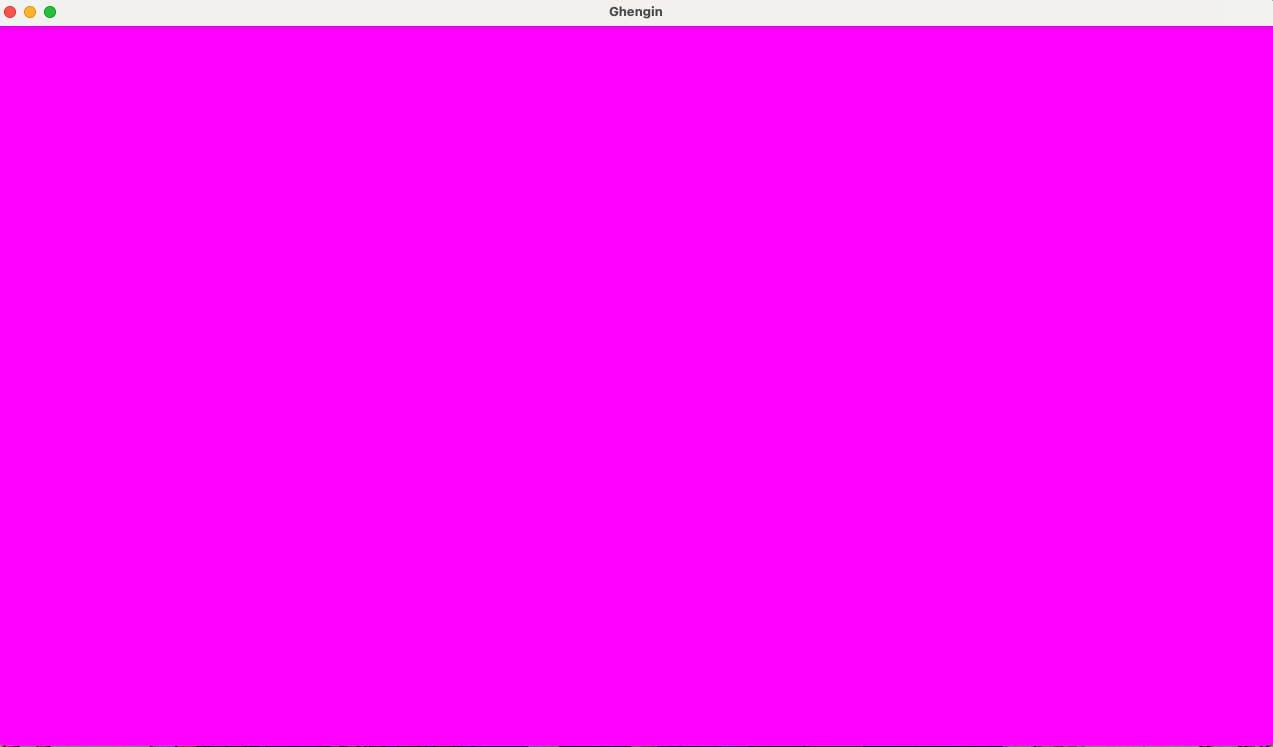
\includegraphics[width=\textwidth]{images/001.png}
\caption{Screaming magenta\label{fig:001}}
\end{figure}


\section{Drawing a plane}

To create an ocean simulation we need a flat plane to define the ocean surface.
An ocean surface is defined by a plane with a number $N$ of equally spaced
particles. We will create all of these particles in their \emph{rest position},
that is, the position they would be in if the ocean was completely flat and
there were no waves. Later on, based on wave math from ``A simple model of
ocean waves''~\cite{10.1145/15886.15894}, every ocean particle's position will
be shifted from its rest position according to time, wind and possibly other
factors.

\subsection{Mesh}

To render an ocean plane we need to create a mesh (see Section~\ref{sec:meshes}
on meshes) that represents one. To create the flat ocean plane we generate $N$
equally spaced \emph{vertices} (see Section~\ref{sec:verts} on vertices). For
now, a vertex is only defined by its position in the world. To make matters
easier, we create type synonyms both for a \text{\ttfamily Position} property (which is really
just a \text{\ttfamily Vec3}), and for the type of \text{\ttfamily Particle} vertices (which are vertices
with one property: a position)

\begin{hscode}\SaveRestoreHook
\column{B}{@{}>{\hspre}l<{\hspost}@{}}%
\column{E}{@{}>{\hspre}l<{\hspost}@{}}%
\>[B]{}\mathbf{type}\;\Conid{Position}\mathrel{=}\Conid{Vec3}{}\<[E]%
\\
\>[B]{}\mathbf{type}\;\Conid{Particle}\mathrel{=}\Conid{Vertex}\;[\mskip1.5mu \Conid{Position}\mskip1.5mu]{}\<[E]%
\ColumnHook
\end{hscode}\resethooks

Then, we define \text{\ttfamily particles}, that takes as input the number of particles to
create in a line and generates the list of vertices that represents the flat
ocean (where $y=0$ always).
\begin{hscode}\SaveRestoreHook
\column{B}{@{}>{\hspre}l<{\hspost}@{}}%
\column{3}{@{}>{\hspre}l<{\hspost}@{}}%
\column{E}{@{}>{\hspre}l<{\hspost}@{}}%
\>[B]{}\Varid{particles}\mathbin{::}\Conid{Int}\to \mathop{}'[\mskip1.5mu \Conid{Particle}\mskip1.5mu]{}\<[E]%
\\
\>[B]{}\Varid{particles}\;\Varid{n}\mathrel{=}[\mskip1.5mu \Conid{Sin}\;(\Varid{vec3}\;\Varid{x}\;\mathrm{0}\;\Varid{z})\mid \Varid{x}\leftarrow [\mskip1.5mu \mathrm{1}\mathinner{\ldotp\ldotp}\Varid{nf}\mskip1.5mu],\Varid{z}\leftarrow [\mskip1.5mu \mathrm{1}\mathinner{\ldotp\ldotp}\Varid{nf}\mskip1.5mu]\mskip1.5mu]{}\<[E]%
\\
\>[B]{}\hsindent{3}{}\<[3]%
\>[3]{}\mathbf{where}\;\Varid{nf}\mathrel{=}\Varid{fromIntegral}\;\Varid{n}\mathbin{::}\Conid{Float}{}\<[E]%
\ColumnHook
\end{hscode}\resethooks


Finally, we create a mesh from the particle vertices. To create a mesh we use
\text{\ttfamily createMesh} which returns a \text{\ttfamily ParticleMesh} which is synonym with \text{\ttfamily Mesh~\char39{}\char91{}Position\char93{}} in the \text{\ttfamily Game} monad. The type of the mesh entails that constituent
vertices have one property which is a \text{\ttfamily Position}.

\begin{hscode}\SaveRestoreHook
\column{B}{@{}>{\hspre}l<{\hspost}@{}}%
\column{E}{@{}>{\hspre}l<{\hspost}@{}}%
\>[B]{}\mathbf{type}\;\Conid{ParticleMesh}\mathrel{=}\Conid{Mesh}\;\mathop{}'[\mskip1.5mu \Conid{Position}\mskip1.5mu]{}\<[E]%
\\[\blanklineskip]%
\>[B]{}\Varid{oceanMesh}\mathbin{::}\Conid{Int}\to \Conid{Game}\;\Conid{ParticleMesh}{}\<[E]%
\\
\>[B]{}\Varid{oceanMesh}\mathrel{=}\Varid{createMesh}\mathbin{\circ}\Varid{particles}{}\<[E]%
\ColumnHook
\end{hscode}\resethooks

\subsection{Material}

A mesh defines the form of an entity, but by itself it cannot describe how
something should be rendered. To render an entity, we need a \text{\ttfamily RenderPacket}. A
render packet is the base unit of renderable entities and each render packet is
formed by a \emph{mesh}, a \emph{material}, and a \emph{render pipeline} which
is compatible with that mesh and material. Section~\ref{sec:renderpacket}
describes render packets in detail.

To get started, we create a material (Section \ref{sec:material}) that simply
defines a base color for all vertices in the mesh associated with that material
in a render packet. The type of the material is parametrized by its properties
which, in this case, are only its color. We define the following synonyms:

\begin{hscode}\SaveRestoreHook
\column{B}{@{}>{\hspre}l<{\hspost}@{}}%
\column{E}{@{}>{\hspre}l<{\hspost}@{}}%
\>[B]{}\mathbf{type}\;\Conid{Color}\mathrel{=}\Conid{Vec3}{}\<[E]%
\\
\>[B]{}\mathbf{type}\;\Conid{OceanMaterial}\mathrel{=}\Conid{Material}\;\mathop{}'[\mskip1.5mu \Conid{Color}\mskip1.5mu]{}\<[E]%
\ColumnHook
\end{hscode}\resethooks

To create the material we will use the \text{\ttfamily material} function as described in
Section~\ref{sec:material}, specifying that the color property is a static
binding which should only be written to explicitly, rather than every frame (in
contrast, a \text{\ttfamily DynamicBinding} is written every frame). The \text{\ttfamily material} function
takes as an argument a \text{\ttfamily RenderPipeline} whose creation we delegate to the
caller of the \text{\ttfamily oceanMat} function. Unfortunately, \text{\ttfamily material} is still coupled
to the Vulkan render backend, so we must lift the \text{\ttfamily Renderer} computation into
\text{\ttfamily Ghengin} using \text{\ttfamily lift}.

\begin{hscode}\SaveRestoreHook
\column{B}{@{}>{\hspre}l<{\hspost}@{}}%
\column{E}{@{}>{\hspre}l<{\hspost}@{}}%
\>[B]{}\Varid{oceanMat}\mathbin{::}\Conid{RenderPipeline}\to \Conid{Color}\to \Conid{Game}\;\Conid{OceanMaterial}{}\<[E]%
\\
\>[B]{}\Varid{oceanMat}\;\Varid{rp}\;\Varid{col}\mathrel{=}\Varid{lift}\mathbin{\$}\Varid{material}\;(\Conid{StaticBinding}\;\Varid{col})\;\Varid{rp}{}\<[E]%
\ColumnHook
\end{hscode}\resethooks

Note that the \text{\ttfamily RenderPipeline} argument has an underscore in front of it. We'll
see that a \text{\ttfamily RenderPipeline} is parametrized by its render information at the
type-level. However, the pipeline info is a complex and large type that
basically describes the whole pipeline, so we do not want to write it out
completely, and the underscore allows us to do just that. The underscore is
called a type hole and makes \text{\ttfamily oceanMat} have a so-called partial type signature
which is possible because of the extension \text{\ttfamily PartialTypeSignatures}. If you
further want to disable warnings regarding partial type signatures you might
add the following lines to the top of your module:

\begin{hscode}\SaveRestoreHook
\column{B}{@{}>{\hspre}l<{\hspost}@{}}%
\column{E}{@{}>{\hspre}l<{\hspost}@{}}%
\>[B]{}\mbox{\enskip\{-\# LANGUAGE PartialTypeSignatures  \#-\}\enskip}{}\<[E]%
\\
\>[B]{}\mbox{\enskip\{-\# OPTIONS\_GHC -Wno-partial-type-signatures  \#-\}\enskip}{}\<[E]%
\ColumnHook
\end{hscode}\resethooks

\subsection{Render and Shader Pipeline}

To create a render pipeline one must first know and think about how game
engines render entities. A render pipeline is one of the most important
concepts in game development with Ghengin (and with any engine really, despite
it often being out of sight until one reaches a high intermediate level). An in
depth explanation of rendering and render pipelines is given in
Section~\ref{sec:rendering} and Section~\ref{sec:renderpipeline}.

In this section, we focus on implementing a render pipeline for our ocean
simulation. The key idea is that every vertex in our ocean mesh will be
processed by a \emph{vertex shader} that may use the properties specified in
the material associated with the ocean mesh, said vertex shader should displace
the vertex according to a wave function that determines the displacement as a
function on the current time and on the vertex position, and, then, every
fragment in the triangles defined by the vertices is processed by a
\emph{fragment shader} that will color the ocean according to the wave height,
lighting, base hue, and other properties.

With that in mind, let's start by creating a new module \text{\ttfamily Ocean\char46{}Shader}. In this
module we will create both our vertex and fragment shader, and define the shader
pipeline. A shader pipeline can then be used as a specification to create a
render pipeline. All shaders must be written using the \text{\ttfamily fir} shader language. We
need the following extensions and imports to write \text{\ttfamily fir} shaders. This is a
natural requirement to using a type-heavy shader language:

\begin{hscode}\SaveRestoreHook
\column{B}{@{}>{\hspre}l<{\hspost}@{}}%
\column{E}{@{}>{\hspre}l<{\hspost}@{}}%
\>[B]{}\mbox{\enskip\{-\# LANGUAGE GHC2021  \#-\}\enskip}{}\<[E]%
\\
\>[B]{}\mbox{\enskip\{-\# LANGUAGE DataKinds  \#-\}\enskip}{}\<[E]%
\\
\>[B]{}\mbox{\enskip\{-\# LANGUAGE RebindableSyntax  \#-\}\enskip}{}\<[E]%
\\
\>[B]{}\mbox{\enskip\{-\# LANGUAGE BlockArguments  \#-\}\enskip}{}\<[E]%
\\
\>[B]{}\mbox{\enskip\{-\# LANGUAGE PartialTypeSignatures  \#-\}\enskip}{}\<[E]%
\\
\>[B]{}\mbox{\enskip\{-\# OPTIONS\_GHC -Wno-partial-type-signatures  \#-\}\enskip}{}\<[E]%
\\
\>[B]{}\mathbf{import}\;\Conid{\Conid{Ghengin}.\Conid{Shader}.FIR}{}\<[E]%
\\
\>[B]{}\mathbf{import}\;\Conid{\Conid{Ghengin}.Shader}{}\<[E]%
\ColumnHook
\end{hscode}\resethooks

Our first vertex shader will do absolutely nothing to the position of the point.
Later we'll revise what should indeed be done, but, for now, we just want to get
something on the screen. The type signature of the vertex shader indicates
what's available in its scope. We define one simple \text{\ttfamily Input} which can be
referenced to by the name \text{\ttfamily in\char95{}position}:
\begin{hscode}\SaveRestoreHook
\column{B}{@{}>{\hspre}l<{\hspost}@{}}%
\column{E}{@{}>{\hspre}l<{\hspost}@{}}%
\>[B]{}\Varid{vertex}\mathbin{::}\Conid{VertexShaderModule}\;\mathop{}'[\mskip1.5mu \text{\ttfamily \char34 in\char95 position\char34}\;(\mathop{}'\cdot \mathbin{:->})\;\Conid{Input}\;\mathop{}'[\mskip1.5mu \Conid{Location}\;\mathrm{0}\mskip1.5mu]\;(\Conid{V}\;\mathrm{3}\;\Conid{Float})\mskip1.5mu]\;\anonymous {}\<[E]%
\ColumnHook
\end{hscode}\resethooks
An \text{\ttfamily Input} to the vertex shader represents a property that all vertices passed
to the input shader. When we previously defined our \text{\ttfamily Mesh} we also had to
specify at the type level the vertex properties. Here it's the same, but at the
shader level. One could even move the type synonyms definitions to this module
and import them from the main module. Additionally, note once again the
underscore for the partial type signature as the last argument to
\text{\ttfamily VertexShaderModule}.

The body of the vertex shader accompanies its type signature. A vertex shader
must output a ``final'' position value (a \text{\ttfamily Vec4}) in the vulkan clip space for
the input vertex. The vulkan clip space is defined by $x\in[-1,1], y\in[-1,1],
z\in[0,1]$.  To do so, we must get the value from the input \text{\ttfamily in\char95{}position} and
output the value by writing to the variable \text{\ttfamily gl\char95{}Position}. In fir, we can get
values from variables, structs and the like using \text{\ttfamily use} combined with a
type-level optic such as \text{\ttfamily Name} (to get a variable by name).

\begin{hscode}\SaveRestoreHook
\column{B}{@{}>{\hspre}l<{\hspost}@{}}%
\column{3}{@{}>{\hspre}l<{\hspost}@{}}%
\column{E}{@{}>{\hspre}l<{\hspost}@{}}%
\>[B]{}\Varid{vertex}\mathrel{=}\Varid{shader}\;\mathbf{do}{}\<[E]%
\\
\>[B]{}\hsindent{3}{}\<[3]%
\>[3]{}\mathord{\sim}(\Conid{Vec3}\;\Varid{x}\;\Varid{y}\;\Varid{z})\leftarrow \Varid{use}\mathord{@}(\Conid{Name}\;\text{\ttfamily \char34 in\char95 position\char34}){}\<[E]%
\\
\>[B]{}\hsindent{3}{}\<[3]%
\>[3]{}\Varid{put}\mathord{@}\text{\ttfamily \char34 gl\char95 Position\char34}\;(\Conid{Vec4}\;\Varid{x}\;\Varid{y}\;\Varid{z}\;\mathrm{1}){}\<[E]%
\ColumnHook
\end{hscode}\resethooks

The fragment shader takes as input the non-built-in outputs of the vertex shader
(in our case, there are no outputs besides the built-in \text{\ttfamily gl\char95{}Position}), and
outputs a final color for that fragment. Additionally, both vertex and fragment
shaders can access values made available through descriptor sets, for example,
the properties defined by a material are made available in descriptor set $1$.
Soon, we will paint every fragment with the base color property passed in the
material. However, we will only see how to access the material color futher
ahead for a surprise reason. For now, we paint every fragment white by setting
the built-in output variable \text{\ttfamily out\char95{}col} with a \text{\ttfamily Vec4}:
% (which is fixed at @Location 0@, so there
% can be no other custom outputs at the same location)

\begin{hscode}\SaveRestoreHook
\column{B}{@{}>{\hspre}l<{\hspost}@{}}%
\column{3}{@{}>{\hspre}l<{\hspost}@{}}%
\column{E}{@{}>{\hspre}l<{\hspost}@{}}%
\>[B]{}\Varid{fragment}\mathbin{::}\Conid{FragmentShaderModule}\;\mathop{}'[\mskip1.5mu \mskip1.5mu]\;\anonymous {}\<[E]%
\\
\>[B]{}\Varid{fragment}\mathrel{=}\Varid{shader}\;\mathbf{do}{}\<[E]%
\\
\>[B]{}\hsindent{3}{}\<[3]%
\>[3]{}\Varid{put}\mathord{@}\text{\ttfamily \char34 out\char95 colour\char34}\;(\Conid{Vec4}\;\mathrm{1}\;\mathrm{1}\;\mathrm{1}\;\mathrm{1}){}\<[E]%
\ColumnHook
\end{hscode}\resethooks

You might note that the fragment shader definitions list is empty. That's
alright, we don't need any additional definition to the built in ones.

To finalize the first shader pipeline iteration, we specify the \text{\ttfamily ShaderPipeline}
which puts together our shader modules (and an additional specification of the
vertex data).

\begin{hscode}\SaveRestoreHook
\column{B}{@{}>{\hspre}l<{\hspost}@{}}%
\column{3}{@{}>{\hspre}l<{\hspost}@{}}%
\column{5}{@{}>{\hspre}l<{\hspost}@{}}%
\column{E}{@{}>{\hspre}l<{\hspost}@{}}%
\>[B]{}\Varid{oceanShaderPipeline}\mathbin{::}\Conid{ShaderPipeline}\;\anonymous {}\<[E]%
\\
\>[B]{}\Varid{oceanShaderPipeline}{}\<[E]%
\\
\>[B]{}\hsindent{3}{}\<[3]%
\>[3]{}\mathrel{=}\Conid{ShaderPipeline}\;(\Conid{StructInput}\mathord{@}(\Conid{ToStructInput}\;\mathop{}'[\mskip1.5mu \Conid{V}\;\mathrm{3}\;\Conid{Float}\mskip1.5mu])\mathord{@}(\Conid{Triangle}\;\Conid{List})){}\<[E]%
\\
\>[3]{}\hsindent{2}{}\<[5]%
\>[5]{}\mathbin{:>->}\Varid{vertex}{}\<[E]%
\\
\>[3]{}\hsindent{2}{}\<[5]%
\>[5]{}\mathbin{:>->}\Varid{fragment}{}\<[E]%
\ColumnHook
\end{hscode}\resethooks

The \text{\ttfamily StructInput} constructor for now requires a bit of boilerplate. We call
\text{\ttfamily ToStructInput} on the list of properties each vertex has (in our case, a vector
of size 3 for the position), specify that our mesh is defined by a triangle list
(currently, this is the only option supported by the engine), and finally wrap
it into a shader pipeline using \text{\ttfamily ShaderPipeline}. The \text{\ttfamily \char58{}\char62{}\char45{}\char62{}} constructor
specifies how the pipeline is connected and to what shader modules.

\text{\ttfamily oceanShaderPipeline} is our shader pipeline which can now be used to construct
a render pipeline. Going back to our \text{\ttfamily Main} module, we \text{\ttfamily import~Ocean\char46{}Shader} and
edit our \text{\ttfamily ini} function to create a render pipeline:

\begin{hscode}\SaveRestoreHook
\ColumnHook
\end{hscode}\resethooks



\include{ocean/Main.tex}

\end{document}

